\documentclass[conference]{IEEEtran}
\usepackage[utf8]{inputenc}
\usepackage{amsmath,amssymb,graphicx,booktabs}

\usepackage[hidelinks,unicode,pdftitle={Extrapolating the Instruct Task Vector of Qwen2.5-0.5B: Scaling lambda Beyond 1 Under Validation-Selected Coefficients on ARC, HellaSwag, and WinoGrande},pdfauthor={Dheiver Francisco Santos},pdfkeywords={task arithmetic, task vectors, extrapolation, model merging, Qwen2.5, paired bootstrap},pdfsubject={Preprint, Figshare, doi:10.6084/m9.figshare.35013988}]{hyperref}
\begin{document}

\title{Extrapolating the Instruct Task Vector of Qwen2.5-0.5B: Scaling $\lambda$ Beyond 1 Under Validation-Selected Coefficients on ARC, HellaSwag, and WinoGrande}

\author{\IEEEauthorblockN{Dheiver Francisco Santos, PhD}
\IEEEauthorblockA{Independent Researcher\\
Maceió, Alagoas, Brazil\\
ORCID: https://orcid.org/0000-0002-8599-9436\\
Preprint, Figshare, 2026, \href{https://doi.org/10.6084/m9.figshare.35013988}{doi:10.6084/m9.figshare.35013988}, CC BY 4.0}}

\maketitle

\begin{abstract}
Task arithmetic adds a scaled task vector, the difference between a fine-tuned and a pre-trained model, to the pre-trained weights. We ask whether extrapolating past the fine-tuned model ($\lambda>1$) improves accuracy when $\lambda$ is chosen on held-out validation data. We scale the instruct task vector of Qwen2.5-0.5B over seven values of $\lambda$ up to 2 and measure macro accuracy on ARC-Easy, ARC-Challenge, HellaSwag and WinoGrande, with 1{,}199 validation items for selection and 3{,}967 disjoint test items. The pre-registered hypothesis, that some $\lambda>1$ beats $\lambda=1$, is not confirmed. The best extrapolated coefficient on validation ($\lambda=1.5$) is $0.78$ percentage points (pp) below the instruct model on test, the primary contrast (95\% bootstrap CI $[-1.60,+0.06]$, $p=0.070$), and $0.38$ pp below the base model, the secondary contrast (CI $[-1.54,+0.82]$). The setting $\lambda=2$ is clearly worse ($-2.28$ pp, CI $[-3.35,-1.16]$), and validation selects $\lambda^\ast=0$, the base model. The test peak at $\lambda=0.75$ is exploratory and indistinguishable from the instruct model. The results cover one 0.5B model pair on knowledge and reasoning benchmarks.
\end{abstract}

\begin{IEEEkeywords}
task arithmetic, task vectors, extrapolation, model merging, Qwen2.5, paired bootstrap
\end{IEEEkeywords}

\section{Introduction}
A fine-tuned language model differs from its pre-trained parent by a vector in weight space. Treating that vector as an object that can be scaled and added is the idea behind task arithmetic \cite{ilharco2022editing}. Scaling by $\lambda<1$ interpolates between the parent and the fine-tuned model; scaling by $\lambda>1$ extrapolates past the fine-tuned model, which amplifies whatever fine-tuning changed. Amplification is attractive: if instruction tuning helps, more of it might help more, at zero training cost.

We test this on the most direct case: Qwen2.5-0.5B and its instruction-tuned release Qwen2.5-0.5B-Instruct \cite{qwen25}, scored on multiple-choice log-likelihood benchmarks. The hypothesis was fixed before any merge was run: some extrapolated $\lambda>1$ yields higher test accuracy than $\lambda=1$. The analysis decouples selection from reporting: $\lambda$ is chosen on a validation split, and the effect is measured on a disjoint test split.

Contributions: (i) a paired, item-level measurement of how test accuracy varies with $\lambda\in[0,2]$ for this pair, with confidence intervals; (ii) the finding that no improvement from extrapolation was detected under validation selection, with a separation of selected curve features from exploratory ones; and (iii) a statement of what the benchmark suite cannot say about instruction following, the purpose of an instruct vector.

\section{Related Work}
\textbf{Task arithmetic.} Task vectors, defined as fine-tuned minus pre-trained weights, can be added, negated and scaled to edit model behavior, where the scaling coefficient is a hyperparameter of the method \cite{ilharco2022editing}. Merging several vectors raises interference between them. TIES-Merging addresses it by trimming small updates and resolving sign conflicts \cite{yadav2023ties}, and DARE by randomly dropping and rescaling delta parameters \cite{yu2023dare}. Adaptive variants learn the coefficients rather than fixing them \cite{yang2023adamerging}, and LoRA-composition methods search coefficients without gradients \cite{huang2023lorahub}. Most of this work searches the coefficient on a bounded range; our focus is the single-vector case with the range deliberately extended past 1.

\textbf{Why linear edits can work.} Task arithmetic in the tangent space argues that weight disentanglement, the property that task vectors act independently of each other, explains when adding vectors works, and that fine-tuning in the linearized model improves it \cite{ortizjimenez2023tangent}. Linear mode connectivity shows that the loss can stay low along a line between two networks that share early training \cite{frankle2020lmc}. Both are statements about neighborhoods. Extrapolating past the fine-tuned endpoint leaves the segment between the two models, and we did not find such a guarantee for language models, so we test it empirically.

\textbf{Language-model vectors, interpolation and extrapolation.} Chat Vector adds the difference between a chat model and its base to a model continually pre-trained in another language to transfer instruction following \cite{huang2023chatvector}. Interpolating between zero-shot and fine-tuned weights reports robustness gains under distribution shift \cite{wortsman2022wiseft}, and interpolating weights fine-tuned on different rewards traces a Pareto front \cite{rame2023rewarded}. Averaging, Fisher-weighted merging and regression-based merging combine models near the segment between them \cite{wortsman2022soups,matena2021fisher,jin2022dataless}. Surveys and a toolkit that implements these operators exist \cite{yang2024survey,goddard2024mergekit}, and a study of merging at scale covers model size and base-model strength \cite{yadav2024matters}. The gap we address: an extrapolation range ($\lambda>1$) for a single instruct vector, evaluated with paired statistics on held-out items under validation-only selection, for a small instruct model.

\textbf{Author's related work.} The author's technical notes cover neighboring topics in language-model training: model merging for capability composition \cite{santos2026modelmergingfo}, parameter-efficient fine-tuning (LoRA, QLoRA, DoRA) \cite{santos2026parametereffic}, knowledge distillation and self-distillation \cite{santos2026knowledgedisti}, mixture-of-experts training and sparse upcycling \cite{santos2026mixtureofexper}, curriculum learning and data-efficient pretraining \cite{santos2026curriculumlear}, synthetic data generation and self-improvement \cite{santos2026syntheticdatag}, direct preference optimization \cite{santos2026directpreferen}, RLAIF and Constitutional AI \cite{santos2026rlaifandconsti}, and RLVR and GRPO for reasoning \cite{santos2026reinforcementl}. This paper instead reports a controlled held-out measurement. In a different domain, the author's JEPA preprint \cite{santos2026collapseresist} uses a similar controlled-comparison style (identical budgets, several seeds, confidence intervals).

\section{Method}
Let $\theta_b$ be the base weights and $\theta_i$ the instruct weights, flattened across all tensors. The task vector and the merged model are
\begin{align}
\tau &= \theta_i-\theta_b, \label{eq:tau}\\
\theta(\lambda) &= \theta_b+\lambda\,\tau. \label{eq:ta}
\end{align}
The relative size of the edit and the selection rules are
\begin{align}
\rho(\lambda) &= \frac{\lVert\theta(\lambda)-\theta_b\rVert}{\lVert\theta_b\rVert}=\lambda\,\rho_1, \label{eq:rho}\\
\lambda^\ast &= \arg\max_{\lambda\in\Lambda}\ \mathrm{Acc}_{\mathrm{val}}\big(\theta(\lambda)\big), \label{eq:select}\\
\Delta(\lambda) &= \mathrm{Acc}_{\mathrm{test}}\big(\theta(\lambda)\big)-\mathrm{Acc}_{\mathrm{test}}\big(\theta(1)\big), \label{eq:delta}
\end{align}
with $\Lambda=\{0,0.5,0.75,1,1.25,1.5,2\}$ and $\rho_1=0.0418$ measured for this pair.

\subsection*{Equations and their meaning}
Eq.~(\ref{eq:tau}) is the difference between the instruct and the base weights: everything instruction tuning changed. Eq.~(\ref{eq:ta}) adds a fraction $\lambda$ of that change to the base: $\lambda=0$ is the base model, $\lambda=1$ is the instruct model, and $\lambda=2$ applies the change twice, going as far past the instruct model as the instruct model is from the base. It is the linear interpolation $(1-\lambda)\theta_b+\lambda\theta_i$ with the coefficient allowed outside $[0,1]$. Eq.~(\ref{eq:rho}) says that the distance from the base grows linearly with $\lambda$; with $\rho_1=0.0418$, the edit has relative norm $0.0628$ at $\lambda=1.5$ and $0.0837$ at $\lambda=2$ (exact by linearity, given $\rho_1=0.04185$; $1.5\rho_1=0.0628$, $2\rho_1=0.0837$). Eq.~(\ref{eq:select}) is the validation rule: pick the coefficient with the highest validation macro accuracy. Eq.~(\ref{eq:delta}) is the paired test difference against the instruct model.

A one-line way to see the hypothesis: write $f(\lambda)=\mathrm{Acc}_{\mathrm{test}}(\theta(\lambda))$. Extrapolation can help only if $f$ is still rising at $\lambda=1$, that is $f'(1)>0$. We estimate the slope with the finite difference $[f(1.25)-f(1)]/0.25$; from the paired difference of Section~\ref{sec:results} it is $-1.3$ pp per unit of $\lambda$ with a 95\% interval $[-3.6,+1.2]$ pp, obtained by dividing the interval of $\Delta(1.25)$ by $0.25$. This is a forward difference over $[1,1.25]$; the curve is concave, so it underestimates the slope at $\lambda=1$. The upper end, $+1.2$ pp per unit, is not negligible, so a slightly positive slope is not excluded.

\section{Experimental Protocol}
\textbf{Models.} Qwen2.5-0.5B (revision \texttt{060db64}) and Qwen2.5-0.5B-Instruct (revision \texttt{7ae5576}), Apache-2.0 \cite{qwen25}; the full hashes are in \texttt{MANIFEST.json}. Merging is done in fp32 on the CPU; the result is copied into a bfloat16 model and evaluated with PyTorch on Apple Silicon (MPS). The model pair is the same as in a LERP study of the same repository, in which $\lambda\in[0,1]$ coincides with the LERP coefficient on a grid of 11 points; here $\lambda=0$ and $\lambda=1$ reuse those cached evaluations.

\textbf{Data and splits.} Multiple-choice log-likelihood scoring in the style of the lm-evaluation-harness \cite{gao2021harness}: ARC-Easy and ARC-Challenge \cite{clark2018arc}, HellaSwag \cite{zellers2019hellaswag} (accuracy normalized by characters) and WinoGrande \cite{sakaguchi2019winogrande} (partial scoring). Primary metric: macro mean of the four accuracies. Disjoint splits (seed 0): validation with 300 items per task (299 for ARC-Challenge; 1{,}199 total), test with 1{,}000 per task (967 for WinoGrande; 3{,}967 total).

\textbf{Selection.} The grid $\Lambda$ was fixed in the pre-registration (extrapolation arm $\{1.25,1.5,2\}$, interpolation arm $\{0.5,0.75\}$, plus the endpoints). Two selection rules use validation only: (R1) $\lambda^\ast$ over all of $\Lambda$ (Eq.~\ref{eq:select}); (R2) the best $\lambda$ within the extrapolation arm $\{1.25,1.5,2\}$, which is the pre-registered question. Test accuracy is computed for every grid point so that the curve can be drawn, but no choice uses it; the test peak is reported as an exploratory observation.

\textbf{Baselines.} The best original model chosen on validation (the base, $\lambda=0$: validation $0.4953$ against $0.4853$ for the instruct model) and the instruct model ($\lambda=1$). Every $\lambda$ has the same validation and test budget.

\textbf{Statistics.} Bootstrap over items, tasks equally weighted: 2{,}000 resamples for a single accuracy, 3{,}000 for paired differences; $p$ two-sided from the bootstrap distribution (B$=$3{,}000: the smallest nonzero two-sided $p$ is $2/3{,}000$). The pre-registration (\texttt{experiments/PREREG.md}) fixed 5{,}000 bootstrap resamples; the analysis used 2{,}000 for a single accuracy and 3{,}000 for paired differences (5{,}000 for per-block NLL differences, Articles 7 and 10). The Bonferroni threshold for the six primary comparisons across Articles 1--6 is $0.05/6=0.0083$; it was added after the pre-registration, whose success rule was a paired 95\% CI above zero. Merges are deterministic, so there is no seed variance; uncertainty is over items only. Success criterion (pre-registered, hypothesis 3): the primary contrast is $\lambda>1$ against $\lambda=1$ (the instruct model), and success requires the lower end of its 95\% interval to be above zero. Deviation from the pre-registration: its general rule takes the best original model (here the base) as the primary baseline, but hypothesis 3 (``$\lambda>1$ can beat $\lambda=1$'') grounds the contrast used here. The contrast counted among the six primary comparisons is the validation-selected $\lambda>1$ ($\lambda=1.5$) against $\lambda=1$; the contrast against the base is secondary. We report both.

\section{Results}\label{sec:results}
Table~\ref{tab:main} and Fig.~\ref{fig:fig03} give the curve. On validation, accuracy decreases from $0.4953$ at $\lambda=0$ to $0.4853$ at $\lambda=1$, then rises slightly to $0.4903$ and $0.4911$ at $1.25$ and $1.5$, and falls to $0.4644$ at $\lambda=2$. On test, accuracy is flat within about $0.5$ pp for $\lambda\in[0,1.25]$ ($0.5021$--$0.5069$), declines to $0.4986$ at $1.5$, and to $0.4836$ at $2$.

\begin{table*}[!t]
\caption{Task arithmetic $\theta_b+\lambda(\theta_i-\theta_b)$ on Qwen2.5-0.5B. Macro accuracy on validation ($n=1199$) and on test ($n=3967$, with 95\% bootstrap CI); the last two columns give the paired test difference to the instruct model ($\lambda=1$) with 95\% CI and two-sided $p$. $\lambda=0$ is the base; $\lambda=1$ is the instruct model.}
\label{tab:main}
\centering\small
\begin{tabular}{lccccc}
\toprule
$\lambda$ & Val & Test [95\% CI] & $\Delta(\lambda)$ vs $\lambda=1$ (pp) [95\% CI] & $p$\\
\midrule
0 (base) & 0.4953 & 0.5025 [0.4875, 0.5174] & $-0.40$ [$-1.41$, $+0.62$] & 0.441\\
0.5 & 0.4936 & 0.5021 [0.4869, 0.5174] & $-0.43$ [$-1.25$, $+0.39$] & 0.288\\
0.75 & 0.4895 & 0.5069 [0.4916, 0.5226] & $+0.05$ [$-0.58$, $+0.71$] & 0.889\\
1 (instruct) & 0.4853 & 0.5064 [0.4909, 0.5220] & $0$ (reference) & ---\\
1.25 & 0.4903 & 0.5032 [0.4881, 0.5188] & $-0.32$ [$-0.91$, $+0.31$] & 0.315\\
1.5 & 0.4911 & 0.4986 [0.4837, 0.5147] & $-0.78$ [$-1.60$, $+0.06$] & 0.070\\
2 & 0.4644 & 0.4836 [0.4686, 0.4989] & $-2.28$ [$-3.35$, $-1.16$] & $<0.001$\\
\bottomrule
\end{tabular}
\end{table*}

\begin{figure}[!t]
\centering
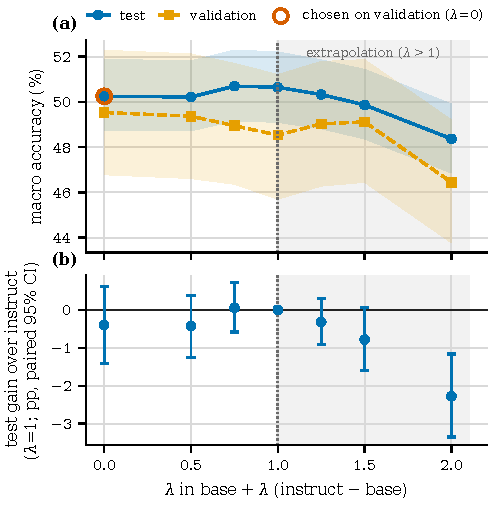
\includegraphics[width=\columnwidth]{figs/fig03_task_arith.pdf}
\caption{(a) Test (solid) and validation (dashed) macro accuracy versus $\lambda$ with 95\% CI bands; the shaded region $\lambda>1$ is extrapolation, and the red ring marks $\lambda=0$, the validation choice. (b) Paired test gain over the instruct model ($\lambda=1$) with 95\% CI.}
\label{fig:fig03}
\end{figure}

\textbf{Pre-registered comparison.} Under R2, validation selects $\lambda=1.5$ among the extrapolated values. Its test macro accuracy is $0.4986$, which is $0.78$ pp below the instruct model (95\% CI $[-1.60,+0.06]$, $p=0.070$) and $0.38$ pp below the base (95\% CI $[-1.54,+0.82]$). The lower end of the interval is not above zero in either comparison, so the hypothesis is not confirmed (primary contrast: against the instruct model; secondary: against the base). The point estimates are negative, but the interval against the instruct model also includes a small positive effect up to $+0.06$ pp. We therefore describe the result as ``no improvement detected for $\lambda\in(1,1.5]$'', not as ``extrapolation hurts'', except at $\lambda=2$.

\textbf{Selection over the whole grid.} Under R1, validation selects $\lambda^\ast=0$ (validation $0.4953$), the base model, which is also the best original model chosen on validation; the difference to the best original is zero because the validation rule returns $\lambda=0$, the base model. The selection rule therefore returns the original model, and no merged model within $\Lambda$ improves on it as measured by validation. (The LERP point $t=0.7$, outside $\Lambda$, has validation $0.4961$ against $0.4953$ for the base; \texttt{cache/q\_lerp\_0.7}.)

\textbf{Degradation at $\lambda=2$.} At $\lambda=2$ the model loses $2.28$ pp against the instruct model (95\% CI $[-3.35,-1.16]$, $p<0.001$) and $1.88$ pp against the base (95\% CI $[-3.17,-0.56]$, $p=0.005$). These two contrasts are post hoc and exploratory, not among the six primary comparisons; both $p$ values would remain below $0.0083$ even if counted among six. On validation the drop from $\lambda=1$ is $-2.08$ pp (95\% CI $[-4.00,-0.08]$, nominal $p=0.045$, not below $0.0083$). We conjecture that this is where the edit ($\rho\approx0.0837$, twice the size of the instruct edit) leaves the region in which weights behave linearly, in the sense of weight disentanglement and mode connectivity \cite{ortizjimenez2023tangent,frankle2020lmc}. We did not test this, and $\lambda=1.75$ or a finer grid might locate the onset.

\textbf{Exploratory: the $\lambda=0.75$ peak.} The highest test accuracy in the grid is at $\lambda=0.75$ ($0.5069$). This is not a selected value: its validation accuracy ($0.4895$) is the fifth highest of seven values, so neither rule R1 nor R2 would choose it, and choosing it after seeing test would be selection on the test set. The advantage is also negligible: $+0.05$ pp over the instruct model (95\% CI $[-0.58,+0.71]$) and $+0.45$ pp over the base (95\% CI $[-0.46,+1.30]$). We report the peak only because it is visible in Fig.~\ref{fig:fig03}; we do not claim that mild under-scaling is beneficial.

\textbf{What cannot be concluded.} First, differences within $[0,1.25]$ are inside the noise: the paired intervals have half-widths of about $0.6$--$1.0$ pp, so smaller effects are not resolved. Second, a flat curve on log-likelihood benchmarks says that extrapolation does not improve knowledge and reasoning accuracy; it does not say that the instruct vector scaled above 1 behaves no better in conversation or instruction following, which these benchmarks do not measure. Third, we have no evidence about other model pairs or scales: the instruct vector of this model is small in relative norm ($0.0418$), and larger or smaller vectors could behave differently.

\section{Discussion and Limitations}
The observed pattern is a plateau followed by a decline. The test curve moves by less than $0.5$ pp between the base and $\lambda=1.25$, and then decreases. No improvement was detected for $\lambda\in(1,1.5]$: $f'(1)$ is not distinguishable from zero, although the interval of $\Delta(1.5)$ reaches $+0.06$ pp and that of the slope reaches $+1.2$ pp per unit of $\lambda$. We conjecture that benchmarks of this kind mostly measure knowledge already present in the base, where instruction tuning adds little. This is consistent with the near-equal accuracy of base and instruct (test $0.5025$ against $0.5064$; instruct minus base $+0.40$ pp, 95\% CI $[-0.62,+1.41]$), but we did not test it with a benchmark that measures instruction following.

The validation set disagrees with the test set about the ordering at the low end: on validation the base is $1.00$ pp above the instruct model (95\% CI $[-0.92,+2.75]$), on test the instruct model is $0.40$ pp above the base. Both differences are inside their intervals. With 1{,}199 validation items, selecting among a few candidates on one split is an instance of adaptive reuse \cite{dwork2015reusable}, and the maximum of noisy scores is biased upward. Therefore the choice of the base model by R1 may be partly noise. For this reason we also report the extrapolation-only rule R2 and the full table, so that readers can apply their own rule.

Threats to validity. (i) One 0.5B model pair, one benchmark family, one hardware setup. (ii) The test split is easier than the validation split, by an amount that differs between models (base $+0.7$ pp, instruct $+2.1$ pp; \texttt{results/summary\_art03.txt}), so gains, not levels, should be compared. (iii) Public benchmarks may be contaminated in the models; this affects all $\lambda$ equally but cannot be measured here. (iv) Merges are deterministic, so seed variance is absent, and the item bootstrap does not reflect variation in the grid. (v) The grid is coarse, and $\{1.25,1.5,2\}$ may miss a narrow useful region such as $1.1$. (vi) The instruct vector bundles supervised fine-tuning with any later alignment stages of the release, and we did not check which of them the log-likelihood benchmarks are sensitive to. All evaluations used bfloat16. Re-evaluating validation accuracy in fp32 at $t=0$, $0.7$ and $1$ (LERP coefficient $t$, equal to $\lambda$ for $\lambda\le1$) lowered the macro accuracy by $0.67$, $0.41$ and $0.08$~pp (fp32: $0.4886$, $0.4920$, $0.4845$), a shift of the same size as the differences between coefficients, while the order of the three points did not change and WikiText-2 NLL moved by at most $0.0026$ nats at any $t$ (\texttt{results/fp32\_check\_qwen.txt}). Exact accuracy levels are therefore specific to bfloat16, and the test items were not re-evaluated in fp32. The validation margin of the base over the instruct model, which supports $\lambda^\ast=0$, falls from $+1.00$ pp (bf16) to $+0.41$ pp (fp32: $0.4886$ against $0.4845$), and in fp32 LERP $t=0.7$ ($0.4920$) exceeds the base ($0.4886$) by $0.34$ pp. The selection of $\lambda^\ast$ is therefore sensitive to precision. fp32 was not measured for $\lambda>1$, the focus of this paper. Paired intervals follow the recommendation of error bars for evaluations \cite{miller2024errorbars}, using the bootstrap \cite{efron1979bootstrap}.

\section{Conclusion}
For Qwen2.5-0.5B, no improvement was detected from scaling the instruct task vector beyond 1 (up to $\lambda=1.5$) in macro accuracy on ARC, HellaSwag and WinoGrande under validation-selected coefficients; the interval of $\Delta(1.5)$ reaches $+0.06$ pp and that of the slope $+1.2$ pp per unit of $\lambda$. The best extrapolated $\lambda$ on validation ($1.5$) is $0.78$ pp below the instruct model on test (95\% CI $[-1.60,+0.06]$). Setting $\lambda=2$ degrades accuracy by $2.28$ pp (95\% CI $[-3.35,-1.16]$), and the full-grid validation rule returns the base model. The pre-registered hypothesis is therefore not confirmed. The test maximum at $\lambda=0.75$ is exploratory and indistinguishable from the instruct model. The natural next tests are an instruction-following benchmark, a finer grid between $1$ and $2$, and other model pairs.

\section*{Data and Code Availability}
\sloppy
Repository: git tag \texttt{preprints-v1} (the commit that contains this manuscript and all scripts and caches). Per-item results are cached in \texttt{cache/} (\texttt{q\_ta\_*}, \texttt{q\_lerp\_0.0}, \texttt{q\_lerp\_1.0}). Single command: \texttt{./run\_everything.sh}; the extra contrasts of this paper (per-$\lambda$ paired differences to the instruct model, comparison to the base) come from \texttt{experiments/\allowbreak an\_art02\_03.py}, written to \texttt{results/extras\_art02\_03.\{json,txt\}}, and the relative norm $\rho_1$ from \texttt{experiments/\allowbreak an\_taskvec.py}. Libraries: Python 3.9.6, PyTorch 2.8.0, transformers 4.57.6, numpy 1.26.4, datasets 4.5.0. Model revisions (Hub commits): Qwen2.5-0.5B \texttt{060db6499f32faf8\allowbreak b98477b0a26969ef7d8b9987}; Qwen2.5-0.5B-Instruct \texttt{7ae557604adf67be\allowbreak 50417f59c2c2f167def9a775}. Pre-registration: \texttt{experiments/PREREG.md}. Raw summary: \texttt{results/summary\_art03.txt}.

\section*{Acknowledgments}
No external funding.

\begin{thebibliography}{99}
\bibitem{ilharco2022editing} G. Ilharco, M. T. Ribeiro, M. Wortsman \emph{et al.}, ``Editing models with task arithmetic,'' in \emph{Proc. ICLR}, 2023. arXiv:2212.04089.
\bibitem{ortizjimenez2023tangent} G. Ortiz-Jimenez, A. Favero, and P. Frossard, ``Task arithmetic in the tangent space: Improved editing of pre-trained models,'' in \emph{Proc. NeurIPS}, 2023. arXiv:2305.12827.
\bibitem{huang2023chatvector} S.-C. Huang, P.-Z. Li, Y.-C. Hsu \emph{et al.}, ``Chat Vector: A simple approach to equip LLMs with instruction following and model alignment in new languages,'' in \emph{Proc.\ ACL}, 2024, arXiv:2310.04799.
\bibitem{wortsman2022wiseft} M. Wortsman, G. Ilharco, J. W. Kim \emph{et al.}, ``Robust fine-tuning of zero-shot models,'' in \emph{Proc. CVPR}, 2022. arXiv:2109.01903.
\bibitem{rame2023rewarded} A. Ram\'e, G. Couairon, M. Shukor \emph{et al.}, ``Rewarded soups: Towards Pareto-optimal alignment by interpolating weights fine-tuned on diverse rewards,'' in \emph{Proc. NeurIPS}, 2023. arXiv:2306.04488.
\bibitem{yadav2023ties} P. Yadav, D. Tam, L. Choshen \emph{et al.}, ``TIES-Merging: Resolving interference when merging models,'' in \emph{Proc. NeurIPS}, 2023. arXiv:2306.01708.
\bibitem{yu2023dare} L. Yu, B. Yu, H. Yu \emph{et al.}, ``Language models are Super Mario: Absorbing abilities from homologous models as a free lunch,'' in \emph{Proc. ICML}, 2024. arXiv:2311.03099.
\bibitem{yang2023adamerging} E. Yang, Z. Wang, L. Shen \emph{et al.}, ``AdaMerging: Adaptive model merging for multi-task learning,'' in \emph{Proc. ICLR}, 2024. arXiv:2310.02575.
\bibitem{huang2023lorahub} C. Huang, Q. Liu, B. Y. Lin \emph{et al.}, ``LoraHub: Efficient cross-task generalization via dynamic LoRA composition,'' in \emph{Proc.\ COLM}, 2024, arXiv:2307.13269.
\bibitem{frankle2020lmc} J. Frankle, G. K. Dziugaite, D. M. Roy \emph{et al.}, ``Linear mode connectivity and the lottery ticket hypothesis,'' in \emph{Proc. ICML}, 2020. arXiv:1912.05671.
\bibitem{wortsman2022soups} M. Wortsman, G. Ilharco, S. Y. Gadre \emph{et al.}, ``Model soups: Averaging weights of multiple fine-tuned models improves accuracy without increasing inference time,'' in \emph{Proc. ICML}, 2022. arXiv:2203.05482.
\bibitem{matena2021fisher} M. Matena and C. Raffel, ``Merging models with Fisher-weighted averaging,'' in \emph{Proc. NeurIPS}, 2022. arXiv:2111.09832.
\bibitem{jin2022dataless} X. Jin, X. Ren, D. Preotiuc-Pietro \emph{et al.}, ``Dataless knowledge fusion by merging weights of language models,'' in \emph{Proc. ICLR}, 2023. arXiv:2212.09849.
\bibitem{yang2024survey} E. Yang, L. Shen, G. Guo \emph{et al.}, ``Model merging in LLMs, MLLMs, and beyond: Methods, theories, applications and opportunities,'' arXiv:2408.07666, 2024.
\bibitem{goddard2024mergekit} C. Goddard, S. Siriwardhana, M. Ehghaghi \emph{et al.}, ``Arcee's MergeKit: A toolkit for merging large language models,'' in \emph{Proc. EMNLP (Industry Track)}, 2024. arXiv:2403.13257.
\bibitem{yadav2024matters} P. Yadav, T. Vu, J. Lai \emph{et al.}, ``What matters for model merging at scale?'' arXiv:2410.03617, 2024.
\bibitem{qwen25} Qwen Team, A. Yang \emph{et al.}, ``Qwen2.5 technical report,'' arXiv:2412.15115, 2024.
\bibitem{clark2018arc} P. Clark, I. Cowhey, O. Etzioni \emph{et al.}, ``Think you have solved question answering? Try ARC, the AI2 reasoning challenge,'' arXiv:1803.05457, 2018.
\bibitem{zellers2019hellaswag} R. Zellers, A. Holtzman, Y. Bisk \emph{et al.}, ``HellaSwag: Can a machine really finish your sentence?'' in \emph{Proc. ACL}, 2019. arXiv:1905.07830.
\bibitem{sakaguchi2019winogrande} K. Sakaguchi, R. Le Bras, C. Bhagavatula, and Y. Choi, ``WinoGrande: An adversarial Winograd schema challenge at scale,'' in \emph{Proc. AAAI}, 2020. arXiv:1907.10641.
\bibitem{gao2021harness} L. Gao \emph{et al.}, ``EleutherAI/lm-evaluation-harness,'' Zenodo, doi:10.5281/zenodo.10256836.
\bibitem{efron1979bootstrap} B. Efron, ``Bootstrap methods: Another look at the jackknife,'' \emph{Ann. Statist.}, vol. 7, no. 1, 1979. doi:10.1214/aos/1176344552.
\bibitem{miller2024errorbars} E. Miller, ``Adding error bars to evals: A statistical approach to language model evaluations,'' arXiv:2411.00640, 2024.
\bibitem{dwork2015reusable} C. Dwork, V. Feldman, M. Hardt \emph{et al.}, ``Preserving statistical validity in adaptive data analysis,'' arXiv:1411.2664, 2014.
\bibitem{santos2026modelmergingfo} D. F. Santos, ``Model Merging for Capability Composition: A Technical Note,'' Zenodo, 2026, doi:10.5281/zenodo.21610555.
\bibitem{santos2026collapseresist} D. F. Santos, ``Collapse-Resistant Joint-Embedding Predictive Architectures: A Controlled Comparison of SIGReg, VICReg, and EMA,'' Zenodo, v2, 2026, doi:10.5281/zenodo.24223364.
\bibitem{santos2026parametereffic} D. F. Santos, ``Parameter-Efficient Fine-Tuning: LoRA, QLoRA, and DoRA,'' Zenodo, 2026, doi:10.5281/zenodo.21610033.
\bibitem{santos2026knowledgedisti} D. F. Santos, ``Knowledge Distillation and Self-Distillation for Language Models,'' Zenodo, 2026, doi:10.5281/zenodo.21610100.
\bibitem{santos2026mixtureofexper} D. F. Santos, ``Mixture-of-Experts Training and Sparse Upcycling,'' Zenodo, 2026, doi:10.5281/zenodo.21610062.
\bibitem{santos2026curriculumlear} D. F. Santos, ``Curriculum Learning and Data-Efficient Pretraining: A Technical Note,'' Zenodo, 2026, doi:10.5281/zenodo.21610595.
\bibitem{santos2026syntheticdatag} D. F. Santos, ``Synthetic Data Generation and Self-Improvement: A Technical Note,'' Zenodo, 2026, doi:10.5281/zenodo.21610525.
\bibitem{santos2026directpreferen} D. F. Santos, ``Direct Preference Optimization (DPO): A Technical Note,'' Zenodo, 2026, doi:10.5281/zenodo.21609911.
\bibitem{santos2026rlaifandconsti} D. F. Santos, ``RLAIF and Constitutional AI: A Technical Note,'' Zenodo, 2026, doi:10.5281/zenodo.21610280.
\bibitem{santos2026reinforcementl} D. F. Santos, ``Reinforcement Learning with Verifiable Rewards (RLVR) and GRPO for Reasoning,'' Zenodo, 2026, doi:10.5281/zenodo.21609980.
\end{thebibliography}

\end{document}
